%
% File emnlp2020.tex
%
%% Based on the style files for ACL 2020, which were
%% Based on the style files for ACL 2018, NAACL 2018/19, which were
%% Based on the style files for ACL-2015, with some improvements
%%  taken from the NAACL-2016 style
%% Based on the style files for ACL-2014, which were, in turn,
%% based on ACL-2013, ACL-2012, ACL-2011, ACL-2010, ACL-IJCNLP-2009,
%% EACL-2009, IJCNLP-2008...
%% Based on the style files for EACL 2006 by 
%%e.agirre@ehu.es or Sergi.Balari@uab.es
%% and that of ACL 08 by Joakim Nivre and Noah Smith

\documentclass[11pt,a4paper]{article}
\usepackage[hyperref]{emnlp2020}
\usepackage{times}
\usepackage{latexsym}
\renewcommand{\UrlFont}{\ttfamily\small}
\usepackage{float}
% This is not strictly necessary, and may be commented out,
% but it will improve the layout of the manuscript,
% and will typically save some space.
\usepackage{microtype}

%\aclfinalcopy % Uncomment this line for the final submission
%\def\aclpaperid{***} %  Enter the acl Paper ID here

%\setlength\titlebox{5cm}
% You can expand the titlebox if you need extra space
% to show all the authors. Please do not make the titlebox
% smaller than 5cm (the original size); we will check this
% in the camera-ready version and ask you to change it back.

\newcommand\BibTeX{B\textsc{ib}\TeX}

\title{Instructions for EMNLP 2020 Proceedings}

\author{First Author \\
  Affiliation / Address line 1 \\
  Affiliation / Address line 2 \\
  Affiliation / Address line 3 \\
  \texttt{email@domain} \\\And
  Second Author \\
  Affiliation / Address line 1 \\
  Affiliation / Address line 2 \\
  Affiliation / Address line 3 \\
  \texttt{email@domain} \\}

\date{}

\begin{document}
\maketitle
\begin{abstract}
As one of the representatives of context word embedding, BERT has achieved the most advanced performance on many NLP tasks. Due to the strong feature extraction ability and the high demand for the amounts of training data, BERT can hardly avoid learning many of the human-generated stereotypes in the text data, including gender bias. In this study, we (1) proposed a template based on language models to quantify gender bias in BERT; (2) proposed a DensRay-based word vector space projection analysis method, which is used in Eliminate gender bias. (3) The method of English training is extended to multilingual BERT, which reduces the gender bias of Chinese on our Chinese template.
\end{abstract}

\section{Introduction}
Word embeddings, which represent the semantic meaning of
text data as vectors, are used as input in natural language
processing tasks. It has been found that word embeddings
exhibit biases such as gender bias, which are present in their training
corpora \cite{bolukbasi2016man,caliskan2017semantics,garg2018word}. Contextual word
embedding models, such as BERT \cite{devlin2018bert}, have
become increasingly common and achieved new state-of-the-art
results in many NLP tasks. Researchers have also found
gender bias in contextualized
embeddings ~\cite{zhao2019gender,may2019measuring}.

A common approach for removing gender information in static
embeddings is to identify a linear gender subspace (e.g., a
gender direction) and subsequently setting all values on the
gender direction to 0. Successful approaches rely on simple
principal component
analysis \cite{bolukbasi2016man,mu2018all}. \newcite{bolukbasi2016man}
require pairs of gendered words to compute a direction
(e.g., ``man''-``woman'') and \newcite{mu2018all} rely on
computing a PCA of a set of gender words hoping that the
main variation occurs across gender. We propose to use
DensRay \cite{dufter2019analytical}: the main advantage is
that DensRay only requires two or multiple groups of
gendered words. In contrast to \cite{bolukbasi2016man}, it
does not require explicit pairs. Compared
to \cite{mu2018all}, it has explicit supervision with gender
labels. We show in \secref{artexample} that this is leads to better gender directions identified by 
DensRay.

In summary, our contributions are: 
i) We adjust DensRay to be usable to debias contextualized embeddings
By evaluating the approach on two tasks, a set of templates we constructed and previously used Association Tests, we show that DensRay performs comparable to prior approaches. 
ii) We provide arguments why DensRay is more robust and find that applying DensRay affects language model performance on downstream tasks less.
iii) We analyse how gender information is processed in BERT by applying DensRay to attention heads and layers: we conclude that there is no single attention head responsible for processing gender information. In addition we show in a qualitative analysis that token-level gender scores can be obtained. 
v) We apply our debiasing method to the multilingual-BERT (mBERT) model: we show that English training data can be used to effectively debias Chinese.



\section{Related Work}
\subsection{The measurements of gender bias}
A typical way to measure gender bias is to evaluate on downstream tasks. For coreference resolution, \citet{zhao2018gender} designed Winobias and \citet{rudinger2018gender} designed Winogender schemas. Different from the WinoBias, Winogender schemas include gender-neutral pronouns which WinoBias doesn't, and one Winogender schema has one occupational mention and one “other participant” mention while WinoBias has two occupational. \citet{webster2018mind} released GAP, a balanced corpus of Gendered Ambiguous Pronouns. Gender bias can be measured as the ratio of F1 score on masculine to F1 score on feminine, however the bias ratios are too close to 1 \citep{Chada_2019, Attree_2019}, so that the bias can't be presented obviously. For sentiment analysis, Equity Evaluation Corpus (EEC) dataset \citep{Kiritchenko_2018} was designed to measure gender bias by the difference in emotional intensity predictions between gender-swapped sentences.

Another kind of method to measure gender bias is based on the association test, it's originated from sociological research. \citet{greenwald1998measuring} proposed the Implicit Association Test (IAT) to quantified societal bias. In the IAT, response times were recorded when subjects were asked to match two concepts. For example, subjects were asked to match black and white names with “pleasant” and “unpleasant” words. Subjects tended to have shorter response times for concepts they thought associated. Based on the IAT, \citet{caliskan2017semantics} proposed the Word Embedding Association Test (WEAT), which used word similarities between targets and attributes instead of the response times to get rid of the reequipment of human subjects. Later, \citet{may2019measuring} extended WEAT to the Sentence Embedding Association Test (SEAT); \citet{kurita2019measuring} proposed a template-based log probability bias score to measure the association between targets and attributes in BERT.

\subsubsection{Word Embedding Association Test}
Here we introduce WEAT in detail. Consider two sets of target words $X_1$ and $X_2$ where $|X_1|=|X_2|$ (equal size) and two sets of attribute words $A_1$ and $A_2$ where $|\mathcal{A}|=|\mathcal{B}|$. As a statistical test, the null hypothesis of WEAT is: There is no difference in the cosine similarity between the $X_1,X_2$ and $
A_1,A_2$. Taking the measurement of gender bias as an example, word sets about science and art can be used as the two target sets, masculine and feminine names can be used as the two attribute sets, such that the null hypothesis means science and art are equally similar to each masculine and feminine names, so there is no gender bias.

The test statistic is defined as,
\begin{eqnarray}
s(X_1,X_2,A_1,A_2)=\sum_{x\in X_1}(x,A_1,A_2)\nonumber\\
-\sum_{x\in X_2}(x,A_1,A_2)\nonumber
\end{eqnarray}
where
\begin{eqnarray}
s(x,A_1,A_2)=mean_{a\in A_1}cos(\vec{x},\vec{a})\nonumber\\
-mean_{a\in A_2}cos(\vec{x},\vec{a})\nonumber
\end{eqnarray}
Intuitively, $s(x,A_1,A_2)$ measures the association of a word with the attributes, so the test statistic measures the differential association of the two target sets with the attributes. 

Let $\{({X_1}_i,{X_2}_i)\}_{i}$ denote all the partitions of $X\cup Y$. The one-sided $p$-value of the permutation test is defined as $$Pr_i[s({X_1}_i,{X_2}_i,A_1,A_2)]>s(X_1,X_2,A_1,A_2)$$
The effect size $d$-value is a normalized measure of how separated the two distributions of associations between the target and attribute are. It is defined as
\begin{eqnarray}
\frac{s(X_1,X_2,A_1,A_2)}{std_{x\in X_1 \cap X_2}s(x,A_1,A_2)}\nonumber
\end{eqnarray}

\subsection{Debiasing methods}
Researchers proposed various methods to remove gender bias, in which the most common way is to define a gender direction (or, more generally, a subspace) by a set of gendered words, and debias the word embeddings in post-processing projecting. \citet{bolukbasi2016man} proposed a hard debiasing method where they used the gendered words to compute the difference embedding vector as the gender direction, and a soft debiasing method which combined the inner-products objective of word embedding and an objective to project the word embedding into a subspace that orthogonal to the gendered words while it performed not so good as the hard debiasing method. \citet{dev2019attenuating} explored partial projection and some simple tricks to improve the hard debiasing method. \citet{zhao2019gender} applied the data augmentation and hard debiasing method of \citet{bolukbasi2016man} to mitigate gender bias on ELMo \citep{Peters:2018}. \citet{karve2019conceptor} introduced the debiasing conceptor, in which they shrined each principal component of the covariance matrix of the word embeddings to achieved a soft debiasing.

\subsection{DensRay}
DensRay is an analytical method proposed to identify the embedding subspace of linguistic features. Here we introduce DensRay for gender debiasing. Same as the methods mentioned in the previous section, we aim to identify the gender bias subspace using a set of gendered words with vocabulary $V:=\{v_1,v_2,\dots,v_n\}$ and embedding matrix $E \in R^{n\times d}$, thus for word $v_i$ we have the corresponding embedding vector $e_{v_i}$. We denotes the gendered words into a map $l:V\to \{-1,1\}$ (e.g. $l(father)=1,l(sister)=-1 $). The objective of DensRay is to find an orthogonal matrix $Q\in R^{d\times d}$ such that $EQ$ is gender-interpretable, specifically, the first $k$ dimensions can be interpreted as the "gender subspace".

Consider $L_{=}:=\{(v,w)\in V\times V|l(v)=l(w)\}$ and $L_{\neq}:=\{(v,w)\in V\times V|l(v)\neq l(w)\}$, we defined $d_{vw}:=e_v-e_w$ as the difference vector of $v$ and $w$. DensRay solves the following optimization problem,
\begin{eqnarray}
    \mathop{max}\limits_{q} 
    \sum_{(v,w)\in L_{\neq}}\alpha_{\neq}||q^Td_{vw}||^2_2\nonumber\\
    -\sum_{(v,w)\in L_{=}}\alpha_{=}||q^Td_{vw}||^2_2
\label{eq:densray1}
\end{eqnarray}
where $q\in R^d$ and $q^Tq=1$ since $Q$ is orthogonal, $\alpha_{\neq},\alpha_{=}\in [0,1]$ are hyperparameters. Intuitively the objective tries to maximize the distance of the word pairs from the same gender group (male words or female words) and minimize the distance of the word pairs from different gender group. Regard that $||x||^2_2=x^Tx$, objective \ref{eq:densray1} can be simplified to:
\begin{eqnarray}
    \mathop{max}\limits_{q} q^T(
    \sum_{(v,w)\in L_{\neq}}\alpha_{\neq}||d_{vw}d_{vw}^T||^2_2\nonumber\\
    \sum_{(v,w)\in L_{=}}\alpha_{=}||d_{vw}d_{vw}^T||^2_2)q\nonumber\\
    =:\mathop{max}\limits_{q} q^TAq
\label{eq:densray2}
\end{eqnarray}

The objective \ref{eq:densray2} is maximizing the Rayleigh quotient of $A$ and $q$. Since $A$ is symmetric, instead of training the model by gradient decent, we can get an analytical solution $q$ by the eigenvector with the max eigenvalue of $A$ \citep{horn1990matrix}. Thus the matrix of $k$ eigenvectors of $A$ ordered by the corresponding eigenvalues yields the matrix $Q$.

\section{Methodology}
\subsection{Debiasing Conceptor}
In this paper, we will compare our work with the debiasing conceptor \cite{karve2019conceptor}. Given a set of gendered words $V:=\{v_1,v_2,\dots,v_n\}$ and their embeddings $E \in R^{n\times d}$, gender bias can be mitigated by multiplying the debiasing conceptor matrix$\neg C= I-C$, where $C$ is the conceptor matrix that minimizes the objective
\begin{eqnarray}
||E-CE||^2_F+\alpha^{-2}||E||^2_F
\end{eqnarray}
where $\alpha$ is a parameter. $C$ has an analytical solution
\begin{eqnarray}
C=\frac{1}{n}EE^T(\frac{1}{n}EE^T+\alpha^{-2}I)^{-1}
\end{eqnarray}
Intuitively, C is a soft projection matrix on the linear subspace where the word embeddings have the maximum bias.

\subsection{Hard Debasing}
We will also compare with the hard debiasing method proposed
by \newcite{mu2018all}, which is originally a postprocessing
technique for improving word
representations. \newcite{karve2019conceptor} adopted it as a
method for debiasing. Hard debiasing relies upon
the assumption that the first principal component of the
embedding vectors is a meaningful gender direction. 
PCA is used to obtain the first
principal component from the embeddings of gendered words
and to project it off.

\subsection{DensRay}
DensRay is an analytical method for identifying the
embedding subspace of certain linguistic features. We aim to
identify the ``gender subspace'' using a set of gendered words
$V:=\{v_1,v_2,\dots,v_n\}$ and their embeddings $E \in
R^{n\times d}$, thus for word $v_i$ we have the
corresponding embedding vector $e_{v_i}$. We
introduce a function $l$ for the gender attribute:
$l:V\to \{-1,1\}$;
e.g. $l(\mbox{father})=1$, $l(\mbox{sister})=-1$. The objective of DensRay
is to find an orthogonal matrix $Q\in R^{d\times d}$ such
that $EQ$ is gender-interpretable, specifically, the first
$k$ dimensions can be interpreted as the gender subspace.

Let $L_{=}:=\{(v,w)\in V\times V|l(v)=l(w)\}$ and define
$L_{\neq}$ analogously.  The DensRay objective
in \eqref{densray1} is to maximize the distance of the word
pairs from the same gender group ($L_{=}$) and minimize the
distance of the word pairs from the different gender group
($L_{\neq}$).
\begin{eqnarray}
\max\limits_{q} 
\sum_{(v,w)\in L_{\neq}}\alpha_{\neq}||q^Td_{vw}||^2_2
-\sum_{(v,w)\in L_{=}}\alpha_{=}||q^Td_{vw}||^2_2
\eqlabel{densray1}
\end{eqnarray}
where we define $d_{vw}:=e_v-e_w$. We also have $q\in R^d$
and $q^Tq=1$ since $Q$ is orthogonal. $\alpha_{\neq},\alpha_{=}\in [0,1]$ are hyperparameters. Observing that $||x||^2_2=x^Tx$, objective \eqref{densray1} can be simplified to:
\begin{eqnarray}
\max \limits_{q} q^T(
\sum_{(v,w)\in L_{\neq}}\alpha_{\neq}||d_{vw}d_{vw}^T||^2_2-\sum_{(v,w)\in L_{=}}\alpha_{=}||d_{vw}d_{vw}^T||^2_2)q=:\max\limits_{q} q^TAq
\eqlabel{eq:densray2}
\end{eqnarray}

This objective is maximizing the Rayleigh quotient of $A$ and $q$. Since $A$ is symmetric, we can get an analytical solution $q$ by the eigenvector with the max eigenvalue of $A$ \cite{horn1990matrix}. Thus the matrix of $k$ eigenvectors of $A$ ordered by the corresponding eigenvalues yields the matrix $Q$.
\subsection{Removing Gender Information}

All prior methods yield a gender dimension $q \in R^d$. In a contextualized language model like BERT each layer yields a contextualized embedding matrix $X \in R^{t \times d}$ where $t$ is the length of the sentence. To debias representations we simply zero out the projected values on $q$ for each position, that is we set $X^{\text{debiased}}_i = X_i -  (X_i^\intercal q) q$ for each position $i$.

\seclabel{artexample}
 \figref{fig:example} shows artificially created two dimensional embeddings. The lines show the gender directions identified by hard debiasing, debiasing conceptor, and DensRay. 
 
 DensRay separates the gendered words into two gender groups to produce a meaningful gender direction by objective \eqref{eq:densray2}, while debiasing conceptor and hard debiasing compute the subspace with the whole gendered words set. Theoretically, they may fail to identify the correct gender direction in some cases. 
\begin{figure}[h]
	\centering
	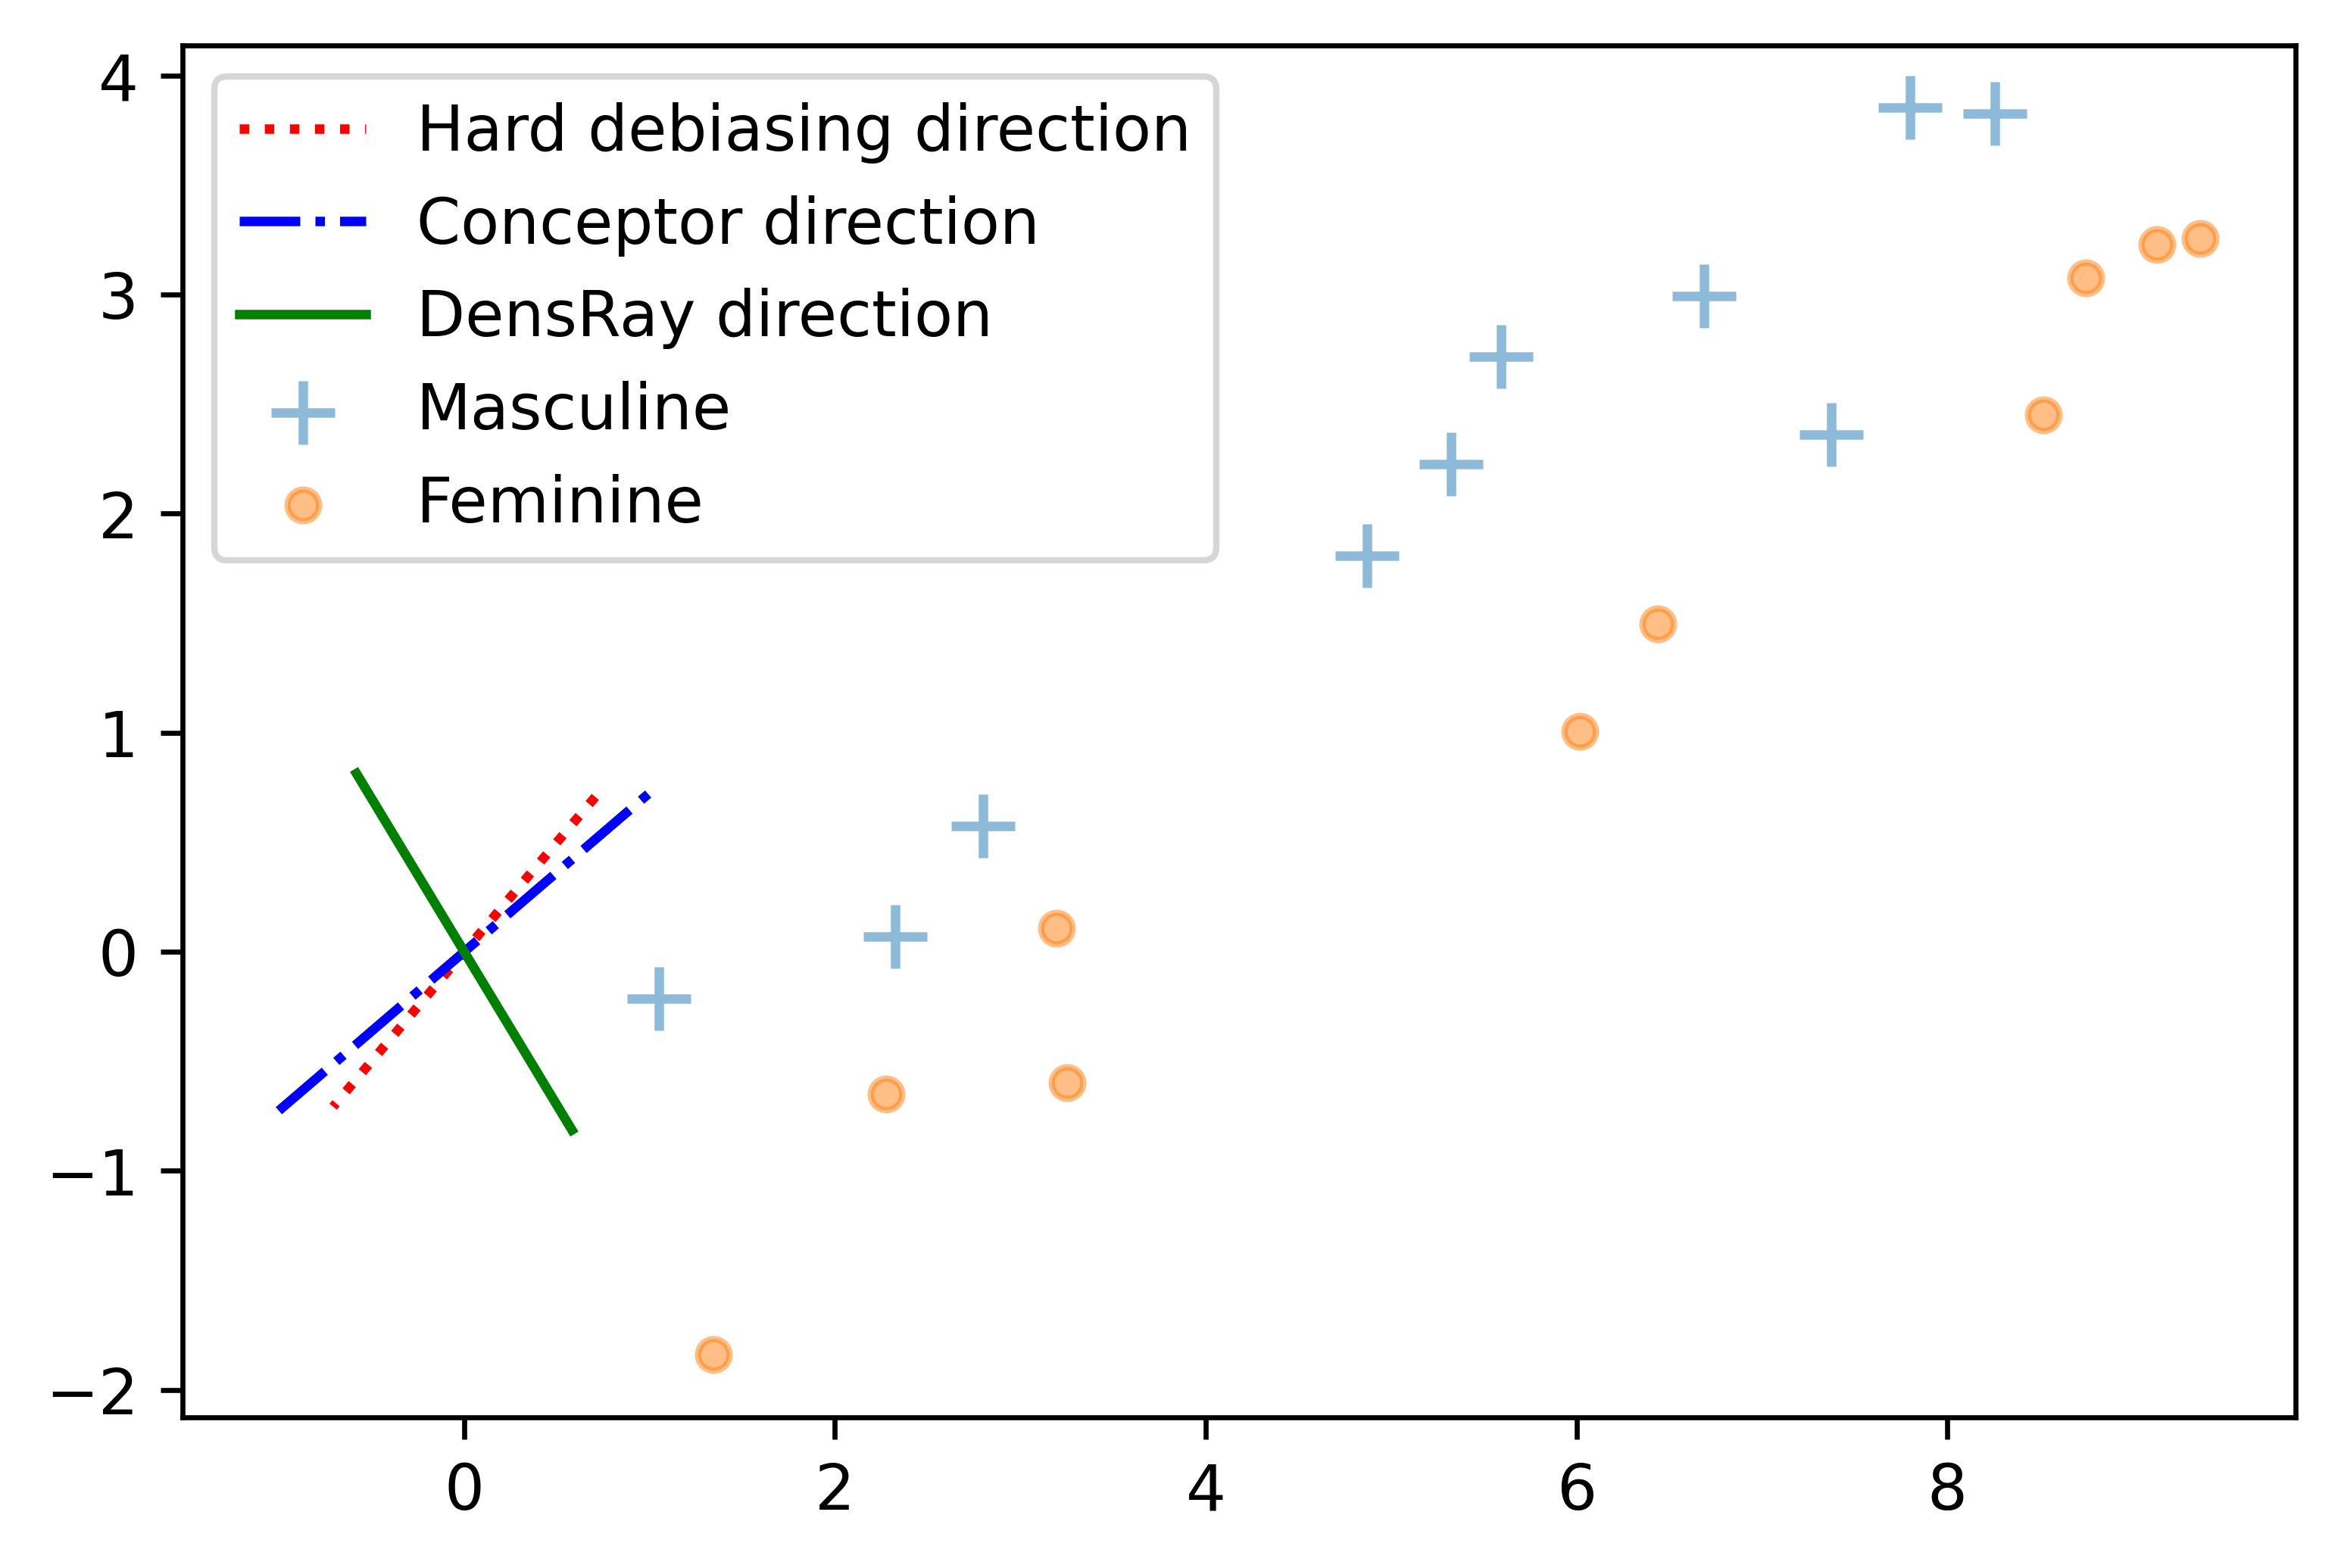
\includegraphics[width=0.5\linewidth]{examples.png}
	\caption{Gender direction on gendered words.}
	\figlabel{fig:example}
\end{figure}

\subsection{Adapting DensRay to Contextualized Language Models}
We now describe how we adapt DensRay to contextualized
language models. Given a set of gendered words
$V$, we extract sentences containing a word in $V$ from a
corpus. We run a contextualized language model
with $M$ layers
on each
sentence
$t_1,\ldots,t_j,\ldots,t_n$ (where $t_j \in V$)
and compute the contextualized representations $e^m, 1\leq m
\leq M$ of $t_j$, one for each layer. 
We compute an orthogonal rotation
matrix $Q_m$ for the $m$th BERT layer using \eqref{eq:densray2}.
For debiasing, we set the gender subspace dimensions to $0$ to eliminate or at least reduce gender information that may cause bias. In this paper, we take the first dimension of the rotated space as the gender subspace.



\section{DensRay Debiasing Experiments on BERT Layers}
\subsection{Experiments Setup}
In the experiments we use the BERT models "bert-base-uncased" and "bert-large-uncased". We implemented all experiments using the transformers library \citep{wolf2019huggingfaces}.

To compute the rotation matrices by DensRay, we need a gendered word list as label, and some corpus. For the word list, we get 23 masculine words and 23 feminine words from the "family" category\footnote{http://download.tensorflow.org/data/questions-words.txt} of the Google analogy test set \citep{mikolov2013efficient}, and label them as 1 and -1. As the input corpus, we collect text data from Wikipedia that contains 5,000 (10,000) occurrences of words in the gendered list. We carefully balance the occurrences such that the number of male and female samples are equal. We set  $\alpha_{\neq}=\alpha_{=}=0.5$, as we have balanced the training samples from the corpus.

\subsection{Results on Templates}
Results about our experiments on the templates are summarized in table \ref{t:templates1}. Two example templates are given in table \ref{t:templates2}. The evaluation on our templates shows that DensRay can mitigate the gender bias on BERT: the average difference between predicting he/she drops by more than half (e.g., bert-base from 0.47 to 0.17)
\begin{table*}[ht]
\centering
\footnotesize
\begin{tabular}{lllll}
\hline
model & prob(he) & prob(she) & diff & var\\
\hline
bert-base & 0.6594 & 0.1874 & 0.4720 & 0.1600 \\
bert-base-densray & 0.5106 & 0.3447 & {0.1658} & 0.0119\\
\hline
bert-large  & 0.6287 & 0.1907 & 0.4380 & 0.1262 \\
bert-large-densray  & 0.4751 & 0.2923 & {0.1827} & 0.0150\\
\hline
\end{tabular}
\caption{ \enote{pd}{I think two digits are sufficient here instead of 4?} \enote{pd}{would be great to use figlabel and figref, or tablabel and tabref}\label{t:templates1}
BERT debiasing results on templates. \textit{bert-base} and \textit{bert-large} are the original model without debiasing. \textit{prob(he)} is the mean probability that model predict \textit{he} as the [MASK]in all templates. \textit{var} is the variance of the differences between the probability of BERT predicts [MASK] as \textit{he} and \textit{she}.}
\end{table*}
\begin{table*}[ht]
\centering
\footnotesize
\begin{tabular}{llll}
\hline
sentence & model & prob(he) & prob(she)\\
\hline
[MASK] is a adjunct professor. & bert-base & 0.7231 & 0.1942\\
 & bert-base-densray & 0.4423 & 0.4740\\
 & bert-large & 0.7181 & 0.2212\\
 & bert-large-densray & 0.3974 & 0.5316\\
\hline
[MASK] is a administrator. & bert-base & 0.6296 & 0.2337\\
 & bert-base-densray & 0.5045 & 0.3762\\
 & bert-large & 0.6456 & 0.2269\\
 & bert-large-densray & 0.4536 & 0.3716\\
\hline
\end{tabular}
\caption{\label{t:templates2}
Two example templates with prediction probabilities.}
\end{table*}

\subsection{Results on WEAT}
In WEAT we measure the effect size $d$-value and the oneside $p$-value of the permutation test. A higher absolute value of the $d$-value indicates larger gender bias between the target words with respect to the attribute words. So, for the $d$-value, the closer to zero, the less gender bias. Refer to the definition of the null hypothesis, if the $p$-value is less than 0.05 we will reject the null hypothesis so that there will be a significant gender bias. So, we would prefer a high $p$-value (at least 0.05) to indicate the lack of gender bias. Follow the same WEAT word lists setup as \citet{karve2019conceptor}, the results on WEAT is shown on table \ref{t:weat1}. For all the three categories, DensRay decreased absolute value of $d$-value and increased the $p$-value, although bert-large still showed strong bias in \textit{(Career, Family) vs (Male, Female)} even after debiasing.
\begin{table*}[ht]
\centering
\footnotesize
\begin{tabular}{llrr}
\hline
category & model & d & p\\
\hline
(Career, Family) vs (Male, Female) & bert-base & 0.6581 & 0.08 \\
                  & bert-base-densray & 0.6397 & 0.11\\
                  & bert-large & 1.5705 & $0.00^{*}$ \\
                  & bert-large-densray & 0.9980 & $0.02^{*}$\\
\hline
(Math, Arts) vs (Male, Female) & bert-base & 0.6017 & 0.11 \\
                  & bert-base-densray & 0.0739 & 0.45\\
                  & bert-large & 0.2239 & 0.35 \\
                  & bert-large-densray & -0.0145 & 0.48\\
\hline
(Science, Arts) vs (Male, Female) & bert-base & 0.7762 & 0.08 \\
                  & bert-base-densray & 0.0167 & 0.49\\
                  & bert-large & 0.816 & $0.04^{*}$  \\
                  & bert-large-densray & 0.6743 & 0.10\\
\hline
\end{tabular}
\caption{\label{t:weat1}
BERT debiasing results on WEAT. * shows significant gender bias.}
\end{table*}

\subsection{Impact on Model Performance}
It is crucial that debiasing methods do not harm downstream performance of BERT models.Thus we test the perplexity of language modeling on the Wikitext-2 dataset \citep{merity2016pointer} which is a subset of Wikipedia with 2 million words, the resuls in table \ref{t:ppl1} show that DensRay caused a small increase in perplexity on Wikitext-2 for both BERT base and large model.
\begin{table}[ht]
\centering
\begin{tabular}{llll}
\hline
model & ppl\\
\hline
bert-base & 3.7714\\
bert-base-densray & 3.8051\\
\hline
bert-large & 3.2928\\
bert-large-densray & 3.3503\\
\hline
\end{tabular}
\caption{\label{t:ppl1}
Language modeling performance on BERT after debiasing with DensRay.}
\end{table}

Following the same setup as \citet{wolf2019huggingfaces}\footnote{https://huggingface.co/transformers/}, we also evaluate on the GLUE tasks \citep{wang2018glue}, results are summarized in table \ref{t:glue1}. 
\begin{table*}[ht]
\centering
\begin{tabular}{llllllllll}
\hline
model & CoLA &SST-2&MRPC&STS-B&QQP&MNLI&QNLI&RTE&WNLI\\
\hline
bert-base & 3.7714& 3.7714& 3.7714& 3.7714& 3.7714& 3.7714& 3.7714& 3.7714& 3.7714\\
bert-base-densray & 3.7714& 3.7714& 3.7714& 3.7714& 3.7714& 3.7714& 3.7714& 3.7714& 3.7714\\
\hline
bert-large & 3.7714& 3.7714& 3.7714& 3.7714& 3.7714& 3.7714& 3.7714& 3.7714& 3.7714\\
bert-large-densray & 3.7714& 3.7714& 3.7714& 3.7714& 3.7714& 3.7714& 3.7714& 3.7714& 3.7714\\
\hline
\end{tabular}
\caption{\label{t:glue1}
GLUE tasks performance on BERT after debiasing with DensRay.}
\end{table*}

\subsection{Discussions}
\subsubsection{Number of training samples}
Through evaluation and inspection of the impact on the performance of downstream tasks, experiments show that DensRay is an effective debiasing method on BERT. Although DensRay is an analytical solution, the effect still depends on size of the training data. In the experiments, we regarded the occurrences of the same word in the corpus as independent words with the same gender label, and used balanced samples for masculine and feminine words. Now we analyze the impact of these processes.

Since there are only 46 words in the gendered word list, if we average their embedding under different contexts, there will be only 46 training samples left for DensRay to calculate. DensRay is essentially a supervised learning method. In the case of insufficient labels, it is difficult for supervised learning to extract useful features. Treating different occurrences as different words greatly enriches training samples. As shown in figure, the debiasing results improve with an increased number of training samples.

The same as other projection-based debiasing methods \citep{bolukbasi2016man,zhao2019gender,dev2019attenuating, karve2019conceptor}, the premise of DensRay debiasing is that the bias direction should be correct. If the sample is unbalanced, the bias direction computed by DensRay will be biased towards either the male or the female, resulting in deleting the gender subspace during debiasing will reverse the gender bias (e.g. there are more masculine words in unbalanced text data, thus the embeddings will be biased towards female after biased). The figure also shows that balanced training sample improved the debiasing performers. 
\begin{figure*}
    \centering
    %\includegraphics{}
    \caption{Here should be a graph.}
    \label{fig:my_label}
\end{figure*}

\subsubsection{Balancing Gender Bias}
In this experiment, we used the method of removing the first dimension (replacing its value by $0$) of the gender interpreteble subspace to remove gender bias. Here we explore some other ways.

In figure \ref{fig:meandebias}, we tried two other ways to remove bias. The first is to replace the first dimension of the gender interpreteble subspace with the mean value of the first dimension of the training samples. The second way is to standardize the first dimension. The results showed that both of these methods did not perform well. We further checked the mean and found that the mean of the different layers is not stable around 0, which is a problem worthy for further exploring.
\begin{figure*}
    \centering
    %\includegraphics{}
    \caption{Here should be a graph.}
    \label{fig:meandebias}
\end{figure*}

As shown in figure \ref{moredim}, we try to delete more dimensions. The results show that removing more dimensions does not improve the debiasing results significantly. \enote{pd}{that is potentially interesting}
\begin{figure*}
    \centering
    \includegraphics{}
    \caption{Here should be a graph.}
    \label{fig:moredim}
\end{figure*}

\subsubsection{Debiasing on different BERT layers}
\enote{pd}{that is interesting to have a graphic, in which layers the most gender bias is contained.}
Here we only apply DesnRay on one BERT layer at a time. We constructed a table to illustrate the top three layers with the best performance on our templates and the three WEAT categories.
\begin{table*}[ht]
\centering
\begin{tabular}{llllllllll}
\hline
\end{tabular}
\caption{\label{t:bestlayers}
Here needs a table.}
\end{table*}



\section{DensRay Debiasing multilingual-BERT}
\subsection{Setup}
As an extension, we apply DensRay to mBERT for zero-shot debiasing on Chinese. Here we use the "bert-multilingual-uncesed" model from \citep{wolf2019huggingfaces}, we also use the same setup as the "bert-base-uncased" model in our previous experiments. 

Still, we compute the rotation matrices by the English gendered words from the "family" category of the Google analogy test set \citep{mikolov2013efficient}.

Since Chinese is a language that doesn't contain genus, we can construct the templates by simply translating from the English templates. After removing the duplicates, we get 302 Chinese templates.

\subsection{Results on Templates}
Results about our experiments on the templates are summarized in table \ref{t:templates2}. Two example templates are given in table \ref{t:templates2}. The evaluation on our templates shows that DensRay can mitigate the gender bias on BERT.
\begin{table*}[ht]
\centering
\begin{tabular}{lllll}
\hline
model & prob(he) & prob(she) & diff & var\\
\hline
bert-multi-en & 0.5064 & 0.1427 & 0.3637 & 0.0619 \\
bert-multi-densray-en & 0.3344 & 0.1207 & 0.2137 & 0.0277 \\
bert-multi-cn & 0.2370 & 0.0718 & 0.1652 & 0.0223 \\
bert-multi-densray-cn & 0.1247 & 0.0407 & 0.0840 & 0.0055\\
\hline
\end{tabular}
\caption{\label{t:templates2}
Results of templates on mBERT after applied DensRay. Models with \textit{-en} are tested on our English templates, and those with \textit{-cn} are tested on our Chinese templates.}
\end{table*}

\begin{table}[ht]
\centering
\begin{tabular}{llll}
\hline
model & ppl\\
\hline
bert-multi & 3.5788\\
bert-multi-densray & 3.7216\\
\hline
\end{tabular}
\caption{\label{t:ppl2}
Language modeling performance on mBERT after applied DensRay.}
\end{table}

We also checked the perplexity for mBERT on Wikitext-2, see table \ref{t:ppl2}. Results show that DensRay can be extended to mBERT as a zero-shot debiasing method for some other languages.

\begin{table*}[t]
\centering
\begin{tabular}{llll}
\hline
sentence & model & prob(he) & prob(she)\\
\hline
[MASK] is a adjunct professor. & bert-multi-en & 0.6823 & 0.1611\\
 & bert-multi-densray-en & 0.5073 & 0.1762\\
& bert-multi-cn & 0.5189 & 0.1108\\
 & bert-multi-densray-cn & 0.3046 & 0.0831\\
\hline
[MASK] is a administrator. & bert-multi-en & 0.5344 & 0.1670\\
 & bert-multi-densray-en & 0.3496 & 0.1318\\
& bert-multi-cn & 0.6823 & 0.1611\\
 & bert-multi-densray-cn & 0.5073 & 0.1762\\
\hline
\end{tabular}
\caption{\label{t:templates3}
Sanity check on the Chinese templates. Here we only present their translation for convenience.}
\end{table*}

\section{Conclusion}
We introduced DensRay debiasing on BERT. Our experiments
showed that this method can effectively mitigate gender bias on OCCTMP and the Association Tests, while maintained the performance of BERT on language modeling and GLUE tasks. We applied DensRay to BERT attention heads, showed that gender information is processed in all attention heads, there is no single attention head responsible for processing gender information. We also used DensRay to obtain interpretable gender bias scores, to quantify bias on token and sentence level for all representations. Finally, we demonstrated that we can remove bias multilingually, we used only English training data to effectively debias Chinese.



%\section*{Acknowledgments}
%
%The acknowledgments should go immediately before the references. Do not number the acknowledgments %section.
%Do not include this section when submitting your paper for review.

\bibliographystyle{acl_natbib}
\bibliography{anthology,emnlp2020}

%\appendix
%\section{Appendices}
%\section{Supplemental Material}
\end{document}
